\chapter{Outils d'analyse de défauts fonctionnels ESD}
\label{chap:4}
\section{Méthode bottom-up}

% What is bottom up
In any bottom-up approach, the study focuses first on the small-scale components of a system.
They are characterized individually, and a model is derived for each component.
Afterwards, these models are assembled together to match the full system architecture.
The main idea of a bottom-up approach is that a system is the sum of its parts.
Ultimately, we study if the robustness of a system can be assimilated as the sum of the robustness of its parts.


% How is it done, core concept
The method described in this section starts by characterizing each block in a particular setup.
This setup provides appropriate biasing to the block, in order to set it in normal operating conditions.
This setup is also in charge of injecting the characterization signal on the tested input, and monitoring of the output under test.
Fig. \ref{block_function_cz} gives an example of such a characterization setup for a supply input.

%TODO: Improve figure (text sizes)
%TODO: Remove range comparator
\begin{figure}[!h]
  \centering
  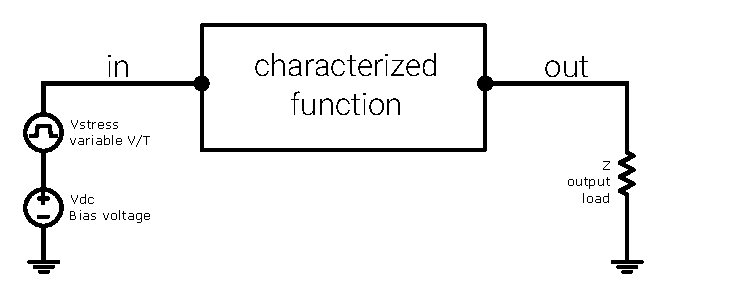
\includegraphics{src/1/figures/characterization_setup.pdf}
  \caption{Block characterization setup (supply input)}
  \label{block_function_cz}
\end{figure}

% What are the characterization signal
The characterization signal is a square waveform, applied on the tested input.
A set of simulations is ran with this setup.
Each simulation runs with a different pair of values for the \textbf{amplitude} and \textbf{duration} of the square signal.
Table \ref{parameterized-simulations} illustrates this simulation process.
In the time domain, this set of simulations is illustrated in Fig. \ref{set_input_signals}.
This testing method was invented by Wunsch and Bell.

%TODO: Fix sim 12 sim12
\begin{figure}[!h]
  \centering
  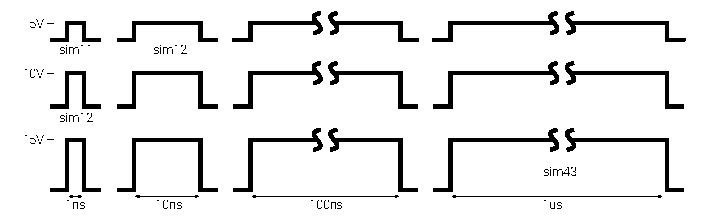
\includegraphics{src/1/figures/time_domain_cz_curves.pdf}
  \caption{Variations on (amplitude, duration) of the input characterization signal}
  \label{set_input_signals}
\end{figure}

The block model contains two 2D tables
The first table still associates an \textbf{output duration} to an input width/amplitude.
The second and new table associates an \textbf{output amplitude} to an input width/amplitude.
Fig. \ref{fig:principle-transfert-func-v2}

Function $F_{W}$ uses the first table mentioned previously, as a \gls{lookup-table}.
It returns for an arbitrary input amplitude and width the closest output width found in the table.
Function $F_{V}$ is identical, except it is using the second table, and returns the closest output amplitude.

\begin{figure}[!h]
  \centering
  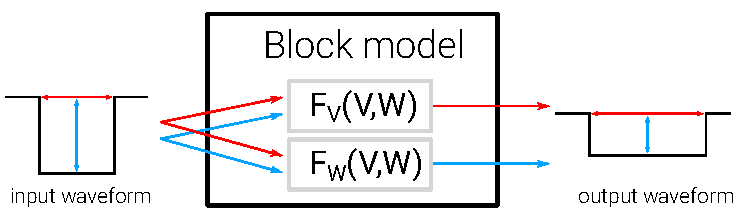
\includegraphics{src/1/figures/principle_transfert_function_v2.pdf}
  \caption{Improved modelling method}
  \label{fig:principle-transfert-func-v2}
\end{figure}

To obtain the response of multiple blocks, models are chained together.

% First run the reference sim
To test this hypothesis, a few simulations are run.
The testbenches are given in Fig. \ref{fig:hypothesis-setup}.
A reference simulation is performed first.
It contains the complete schematic, composed of the three blocks of our study case.
An electrical disturbance is injected on the first input $V_{batt}$.
The final output $V_{2p5}$, and intermediate nets $V_{clamp9}$ and $V_{1p0}$ are observed and disturbance properties on those nets recorded.

\begin{figure}[!h]
  \centering
  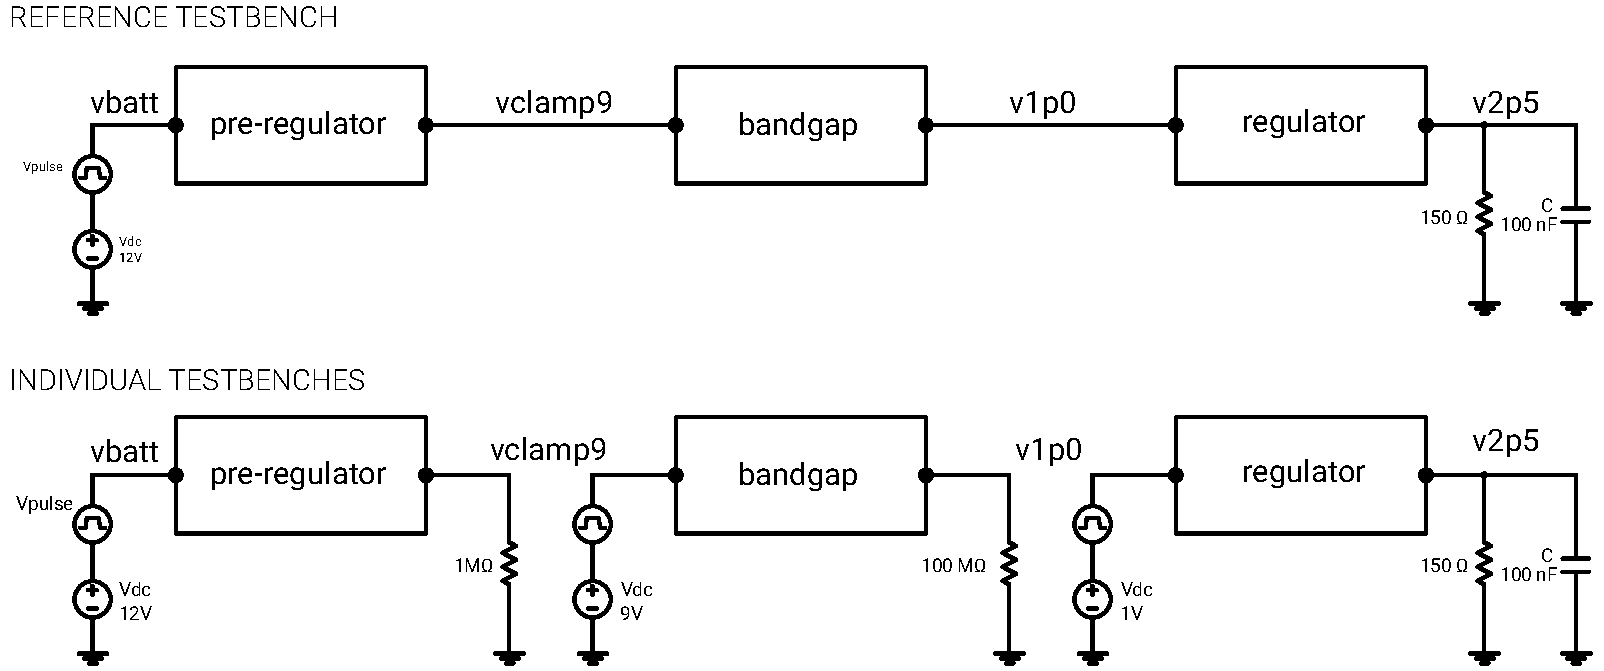
\includegraphics[width=0.98\textwidth]{src/1/figures/hypothesis_testing_setup.pdf}
  \caption{Testbenches used for characterization and hypothesis testing}
  \label{fig:hypothesis-setup}
\end{figure}

% Then do the same thing but with the individual models
Afterwards, each block is simulated separately in its own individual testbench.
The pre-regulator is stressed with the same pulse than the reference simulation.
Its output waveform is compared with the reference in Fig. \ref{fig:sim-compare-block1}.
Both curves (blue and green) look rather similar, in terms of maximum amplitude, duration and overall shape.
The maximum amplitude is estimated at -1.5 V and the duration at 880 ns.
The red curve represents the waveform injected on the second block and configured from these two values.

\begin{figure}[!h]
  \centering
  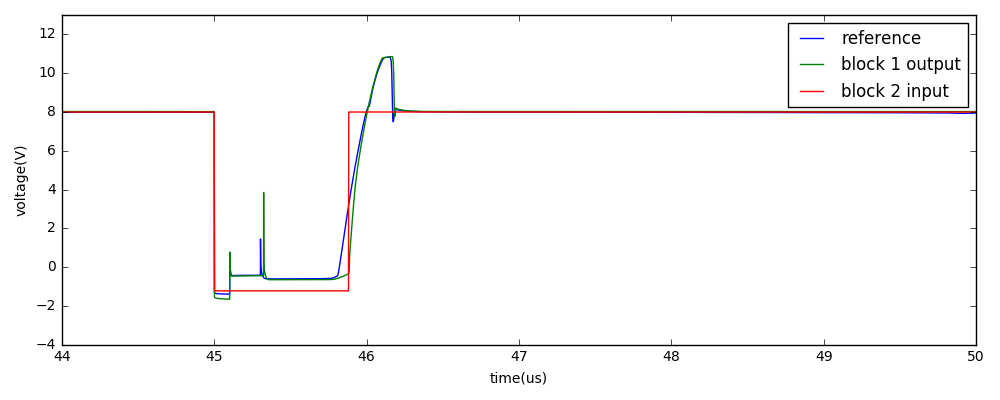
\includegraphics[width=0.98\textwidth]{src/1/figures/simulation_comparison_block1.png}
  \caption{$V_{clamp9}$ waveform}
  \label{fig:sim-compare-block1}
\end{figure}

% Second block output
On the second block output, the blue and green waveforms exhibit more differences (Fig. \ref{fig:sim-compare-block2}).
The green waveform has a longer slope than the reference.
However, both waveforms are still quite close in terms of maximum amplitude and duration.
This is an interesting result, because it shows that \textbf{blocks can be simulated individually} for \gls{esd} simulations, without loosing too much accuracy.
This is great for simulation speed and modularity.
Once again, the red curve represents the waveform injected on the third block.
It is a simplified waveform derived from the blue and green curves, with a width of 2 \textmugreek{}s and an amplitude of 0V.

\begin{figure}[!h]
  \centering
  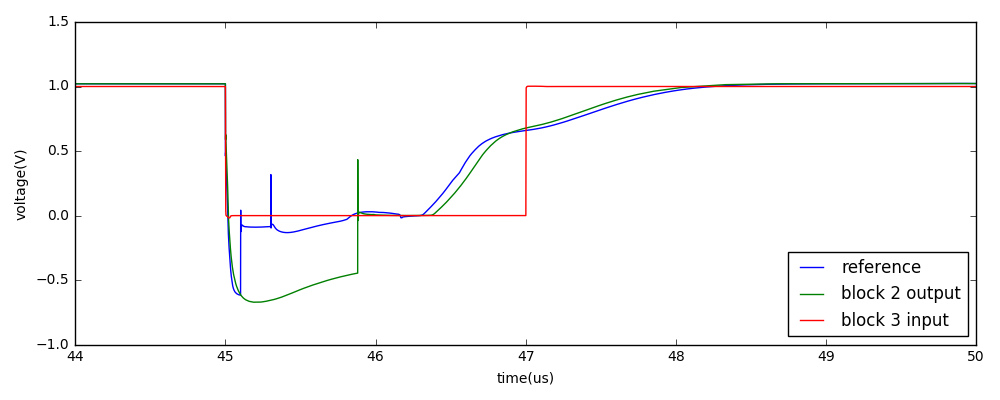
\includegraphics[width=0.98\textwidth]{src/1/figures/simulation_comparison_block2.png}
  \caption{$V_{1p0}$ waveform}
  \label{fig:sim-compare-block2}
\end{figure}

% Third output
On the third and final block output (Fig. \ref{fig:sim-compare-block3}), both waveforms are very similar.
The difference of maximum amplitude can be explained by an offset between both curves at $t=0$.
The reference curve is delayed in comparison of the individual simulation, but otherwise both curves match.

\begin{figure}[!h]
  \centering
  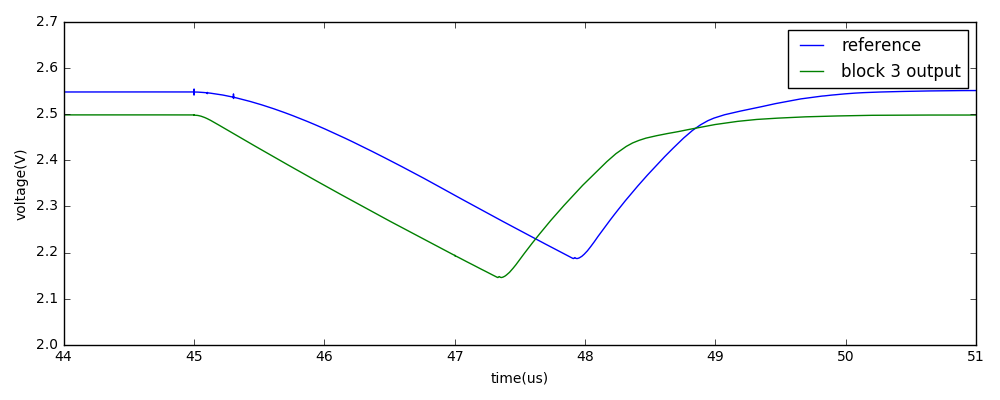
\includegraphics[width=0.98\textwidth]{src/1/figures/simulation_comparison_block3.png}
  \caption{$V_{2p5}$ waveform}
  \label{fig:sim-compare-block3}
\end{figure}

% Conclusion, it works for this case
In conclusion, for this specific study-case, the initial hypothesis was correct.
Simulating the models isolately produced the same results than the reference simulation, for estimating degradation of functionality.
As a consequence, block models extracted from variable amplitude/width characterization should work properly, since it is mathematically equivalent to the simulations that were performed in this section.
block models are simply pre-computed simulations with results stored in \gls{lookup-table}s.

\section{Méthode boite noire}


% Difference with bottom-up, not the same application, not the same goal
The black-box modeling method relies on the same core principles than the bottom-up modeling approach.
It studies the relationship and transfert function between the input and the output of a silicon function.
Unlike the bottom-up method though, the model is only built for external input and output pins.
It is not meant to be chained with other models, using a special chaining method.
Instead, it targets electrical, board-level circuit simulations.
Basically, the black box model is intented to act as a drop-in replacement for the complete \gls{ic} circuit, for board-level simulations.

% introduction, failure relation between input and output
The main benefit of this model is to abstract the internal silicon complexity.
The model focuses on describing the failure of an output when an input is stressed.
At board-level, failure criteria can be more easily set from the chip specification.
After setting the failure criteria, the approach is to inject rectangular pulses on an input pin, and record when an output is in fault.


% How is the characterization conducted
Once again, a variable width/variable amplitude rectangular pulses are applied on an input pin.
The output pin is then observed to detect for which input parameters it is going out of specification.

% What is characterized
This characterization is performed on the testchip, on the complete regulation function.
The characterization pulses are injected on the $V_{batt}$ input.
The output pin is $V_{2p5}$, the regulated supply.
It is supposed to deliver a 2.5V regulated supply.
The failure criteria is set at a voltage below 2.1V.
It corresponds to a level below which digital cells powered by this supply will have noise margins too small for proper operation.

% Fig X shows the waveform of the VBAT injected current when stressed with a TLP (square) impulse.
% The TLP waveform before the capacitor is shown for reference.
%TODO: WAVEFORM CURRENT VBAT AND TLP BEFORE INJECTION CAPACITOR ?

% Detail the characterization
The characterization table is plotted in Fig. \ref{fig:cz-black-box}.
X-axis is the pulse width, and y-axis is the minimal stress amplitude that caused a failure on the output.

\begin{figure}[!h]
  \centering
  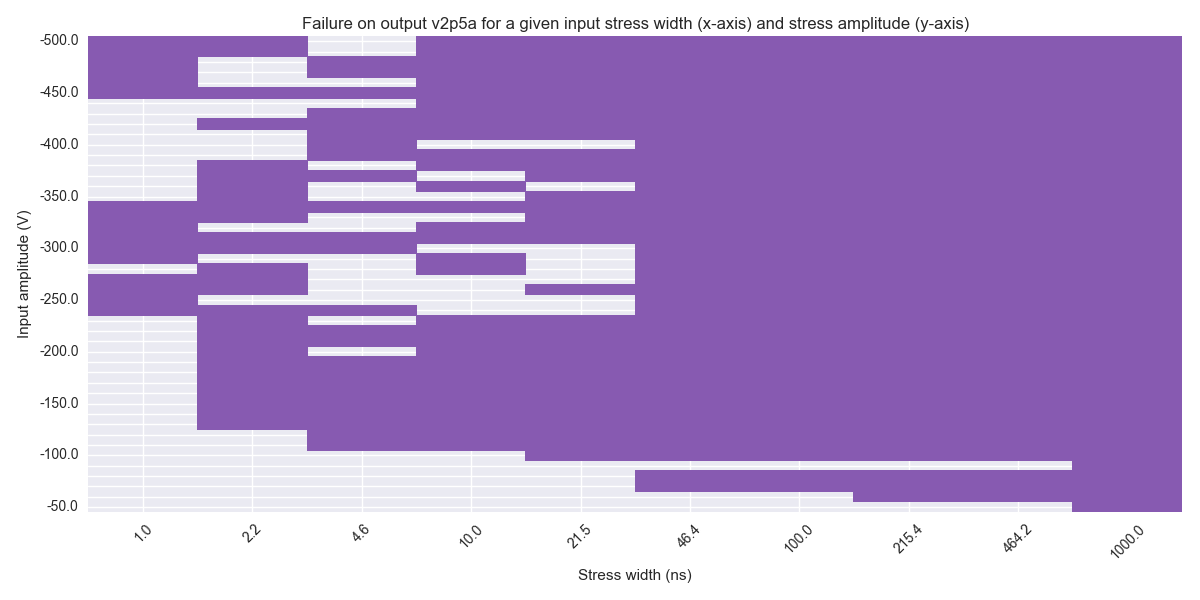
\includegraphics[width=\textwidth]{src/1/figures/black_box_regulator.png}
  \caption{Black-box characterization of the regulation function}
  \label{fig:cz-black-box}
\end{figure}

% What to do with that
%TODO: We that below this value the function is in fail, etc
However, the motivation for this model is to replace the transistor-level schematic inside a SPICE simulation at board-level.
Given a pulse width and an amplitude on $V_{batt}$, the model can estimate the disturbance amplitude and width on $V_{2p5}$.
However, the model itself is not an electrical model, only a failure model.
It cannot determinate, given for instance an input voltage, how much current is flowing into it.
This is also true for the output.
Thus, this method calls for an electrical model of \gls{io}.

\gls{tlp} characterizations are performed on the testchip's regulation function, in powered and unpowered conditions.
For powered conditions, it is considered that full functionality and performance does not matter, just the equivalent impedance of the input or output.
As a consequence, the function is biased but external devices are not connected.
Unpowered and powered characterizations are compared respectively in Fig. \ref{fig:tlp-input-cz} and \ref{fig:tlp-output-cz}.

\begin{figure}[!h]
  \centering
  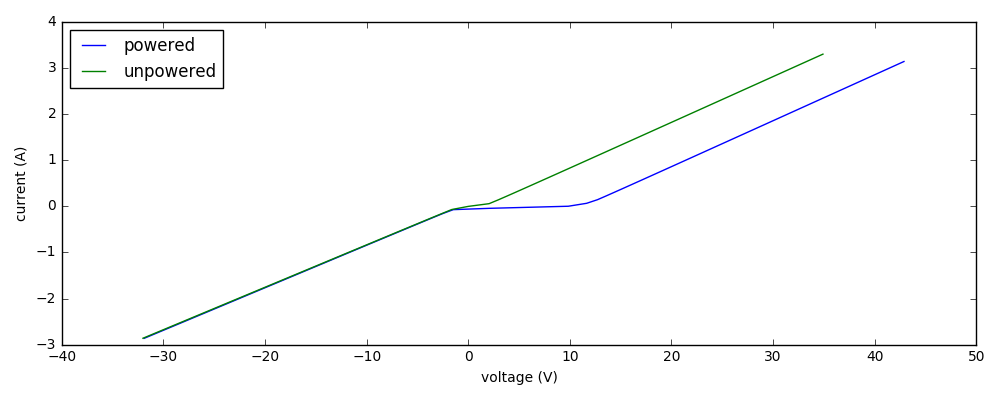
\includegraphics[width=\textwidth]{src/1/figures/tlp_input_characterization.png}
  \caption{TLP characterization of function input in powered and unpowered conditions}
  \label{fig:tlp-input-cz}
\end{figure}

\begin{figure}[!h]
  \centering
  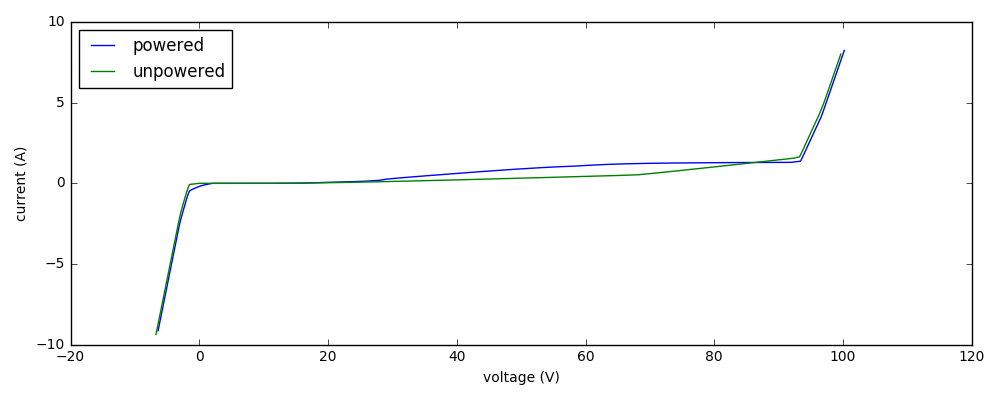
\includegraphics[width=\textwidth]{src/1/figures/tlp_output_characterization.png}
  \caption{TLP characterization of function output in powered and unpowered conditions}
  \label{fig:tlp-output-cz}
\end{figure}


For both input and output ports, large differences are observed between powered and unpowered modes.
Different amount of current are absorbed by the device in each conditions.
Since the model is intended for powered-on simulations, the characterization in powered conditions is chosen.

% Explain the PWL model
The second step of the modelling method is to build an electrically simulatable model of the function.
A piecewise linear model seems well suited for this situation.


% Validate the model with TLP
The verilog-a model is first tested against the complete schematic for the function's input.
After issues described previously were solved, good agreement is achieved between model and complete circuit.
This was verified at -10V, 20V and 40V TLP amplitude (Fig. \ref{fig:compare-model-simu-m10}, Fig. \ref{fig:compare-model-simu-20}, Fig. \ref{fig:compare-model-simu-40}).
The model is considered mostly valid for the input.

\begin{figure}[!h]
  \centering
  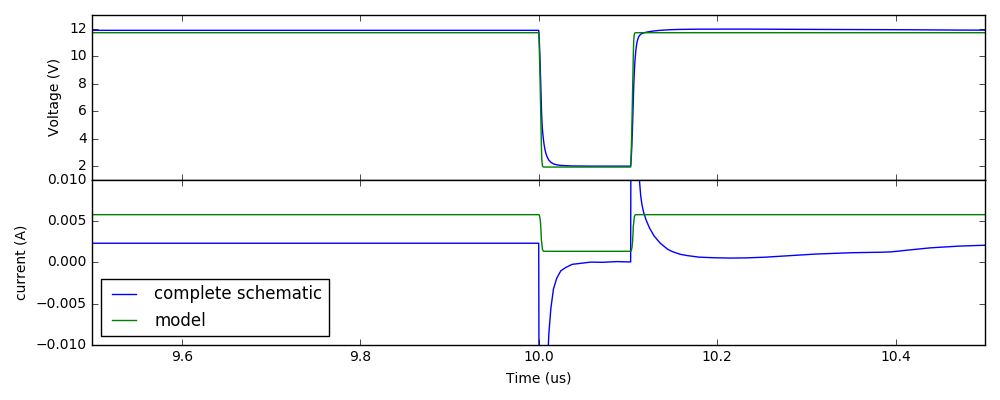
\includegraphics[width=\textwidth]{src/1/figures/comparison_model_total_m10V.png}
  \caption{Comparison of complete schematic and model simulations - -10V TLP}
  \label{fig:compare-model-simu-m10}
\end{figure}


% Check the output
The same test is performed for the function's output model.
The situation is more complex in this case.
The output model must perform three tasks.
First, offer an output impedance close the the one of the real function.
Second, provide a DC value, here corresponding to the regulated 2.5V.
Lastly, reproduce the function reset where the output voltage falls down then restarts.
A first output model is envisionned (Fig. \ref{fig:first-output-model}).

\begin{figure}[!h]
  \centering
  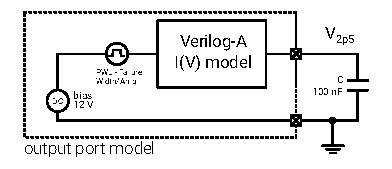
\includegraphics[width=0.3\textwidth]{src/1/figures/first_output_model.png}
  \caption{First proposal for modeling function output}
  \label{fig:first-output-model}
\end{figure}

% Is this first model working
Preliminary and extended tests show that this configuration is not working.

%TODO: Du coup on fait quoi ?


% Conclusion
Black box models of analog integrated functions are very interesting for distributing SPICE models to external parties.
They do not disclose the internal design of the chip, yet they can help achieve system-level ESD simulations.
Ultimately, the goal is to follow the SEED (TODO: Ref) methodology, that indicates that ESD robustness should not be handled at a single level of a system, but at every level (equipment, board, integrated circuit), and that all levels should work efficiently together toward that goal.
Black box models fit very nicely in this methodology.
In this section, a first technique for extracting and creating black-box models was presented.
There is a lot of room for improvements, but it is already working for some intermediate complex cases.
The core principle is that TLP characterization of inputs and ouputs on a biased function is sufficient to extract an equivalent impedance.
This impedance can replace the function in the schematic, during an ESD simulation, in order to reduce complexity and simulation time.
The second core principle is to simplify waveforms into rectangular ones in order to reduce the complexity of the problem.

% Opening work
There are many new leads to explore on these black box models.
First, behavior of the models against more time-varying disturbances such as ESD gun waveforms should be investigated.
Also, the piecewise-linear models should be improved to be more stable, and to fit more closely the extracted I(V) curve.
This technique should be applied to a wider number of analog functions, to observe if it can be used in a general manner.
For now, input and outputs must be simulated separately.
First, the input is simulated, then analyzed to extract the width and amplitude of the disturbance.
This data is then used to configure the output failure source pulse.
The model must be improved in order for the output to react in real-time to the disturbance of the input.
Ultimately, this calls for a Verilog-A model of the failure for instance, plus most likely an improved characterization method able to extract and describe this real-time behavior.
